\documentclass[10pt]{standalone}
\usepackage[utf8]{inputenc}
\usepackage{pgfplots}
\pgfplotsset{compat=1.15}
\usepackage{mathrsfs}
\usetikzlibrary{arrows}
\pagestyle{empty}
\begin{document}
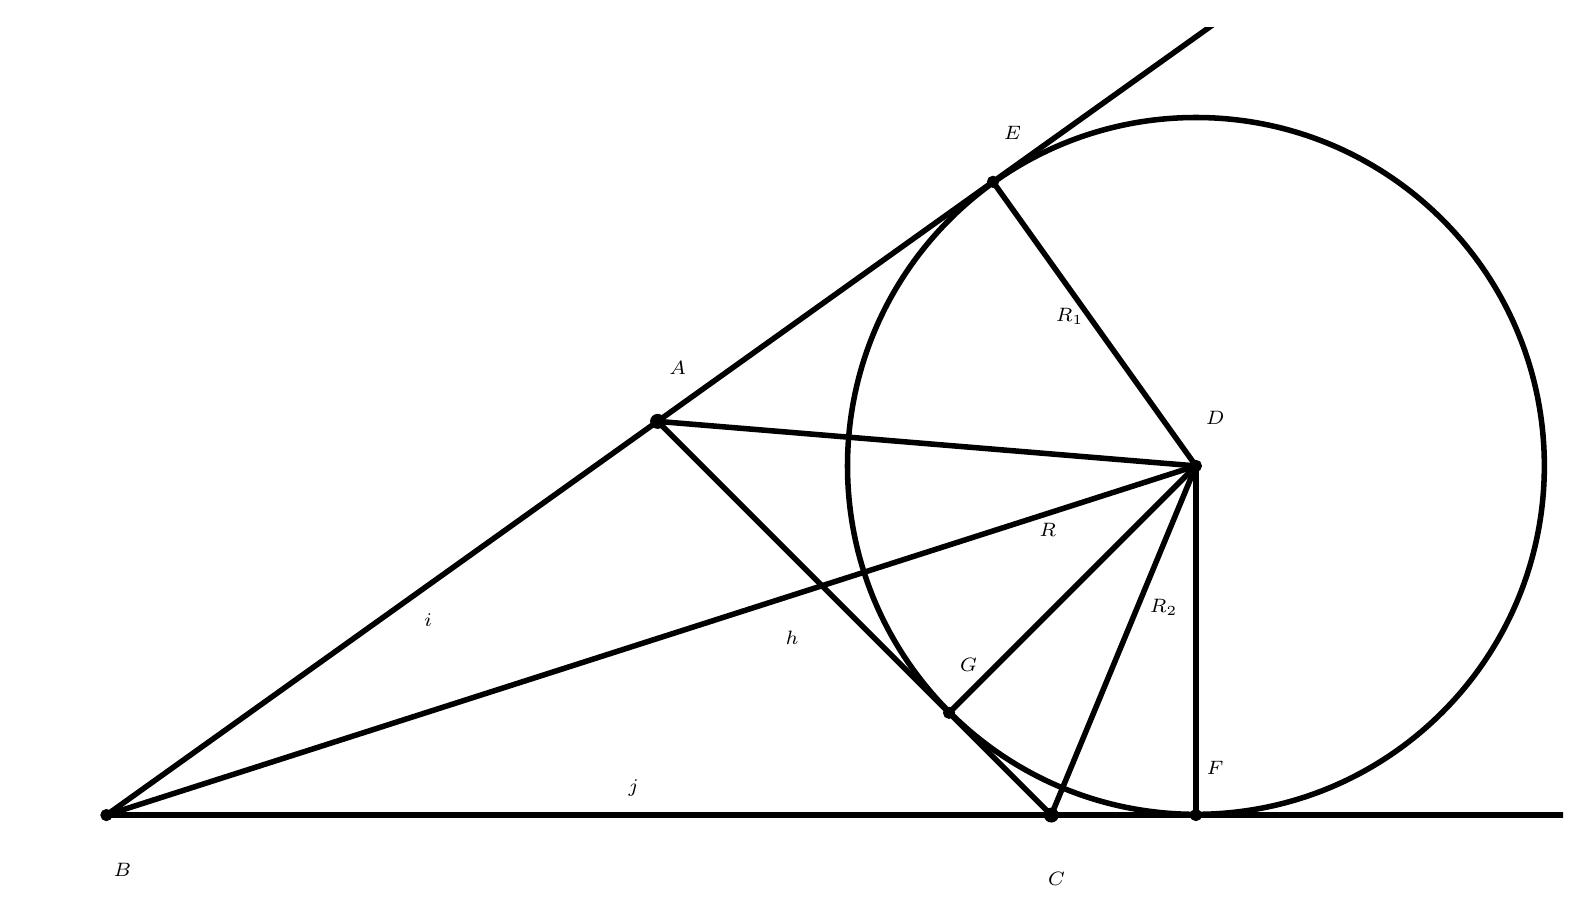
\begin{tikzpicture}[line cap=round,line join=round,>=triangle 45,x=1.0cm,y=1.0cm]
\clip(-1.,-1.) rectangle (18.5,10.);
\draw [line width=2.pt] (12.,0.)-- (7.,5.);
\draw [line width=2.pt,domain=0.0:18.5] plot(\x,{(-0.--5.*\x)/7.});
\draw [line width=2.pt,domain=0.0:18.5] plot(\x,{(-0.-0.*\x)/12.});
\draw [line width=2.pt] (13.83669653945405,4.4341776955137) circle (4.424931549999381cm);
\draw [line width=2.pt] (0.,0.)-- (13.83669653945405,4.4341776955137);
\draw [line width=2.pt] (11.259383105084162,8.042416503631543)-- (13.83669653945405,4.4341776955137);
\draw [line width=2.pt] (13.83669653945405,4.4341776955137)-- (13.836696539454051,0.);
\draw [line width=2.pt] (7.,5.)-- (13.83669653945405,4.4341776955137);
\draw [line width=2.pt] (13.83669653945405,4.4341776955137)-- (12.,0.);
\draw [line width=2.pt] (13.83669653945405,4.4341776955137)-- (10.701259421970173,1.2987405780298258);
\begin{scriptsize}
\draw [fill=black] (7.,5.) circle (2.5pt);
\draw[color=black] (7.254178633946865,5.678290329015679) node {$A$};
\draw [fill=black] (0.,0.) circle (2.0pt);
\draw[color=black] (0.20420774799209745,-0.7002547582767393) node {$B$};
\draw [fill=black] (12.,0.) circle (2.5pt);
\draw[color=black] (12.066063524360436,-0.8121590580537992) node {$C$};
\draw[color=black] (8.70893453104864,2.2465584691858402) node {$h$};
\draw[color=black] (4.08355680693017,2.47036706873996) node {$i$};
\draw[color=black] (6.694657135061566,0.3441853729758206) node {$j$};
\draw [fill=black] (13.83669653945405,4.4341776955137) circle (2.0pt);
\draw[color=black] (14.080340920347512,5.04416596361234) node {$D$};
\draw [fill=black] (11.259383105084162,8.042416503631543) circle (2.0pt);
\draw[color=black] (11.506542025475136,8.66240498973728) node {$E$};
\draw [fill=black] (13.836696539454051,0.) circle (2.0pt);
\draw[color=black] (14.080340920347512,0.6052954057889606) node {$F$};
\draw[color=black] (12.233919974026026,6.33106541104853) node {$R_{1}$};
\draw[color=black] (13.427565838314663,2.63822351840555) node {$R_{2}$};
\draw [fill=black] (10.701259421970173,1.2987405780298258) circle (2.0pt);
\draw[color=black] (10.947020526589837,1.9108455698546605) node {$G$};
\draw[color=black] (11.954159224583375,3.6267114997695797) node {$R$};
\end{scriptsize}

\end{tikzpicture}
\end{document}